\section{Элементы теории четырёхпольсников}
\sectionmark{Элементы теории четырёхпольсников}

Как  известно,  четырёхпольсник  на  фиксированной  частоте характеризуется четырьмя в общем случае комплексными величинами. Эти величины  связывают  токи  и  напряжения на зажимах четырёхполюсника. В зависимости  от  того  какие  параметры  являются  входными  а  какие выходными,  существует  несколько  систем  параметров.  В  данном  случае интерес  представляет  система  А-параметров.  Взаимосвязь  между  токами  и напряжениями в данном случае выражается системой~(\ref{eq:1}) : 


\begin{equation}
\label{eq:1}
\begin{aligned}
 \begin{cases}
\dot{U_{1}} = A_{11}\dot{U_{2}} + A_{12}\dot{I_{2}}\\
\dot{I_{1}} = A_{21}\dot{U_{2}} + A_{22}\dot{I_{2}}
 \end{cases}
\end{aligned}
\end{equation}


или в матричной форме: 


\begin{equation}
\label{eq:1a}
\begin{aligned}
\begin{bmatrix} \dot{U_{1}} \\ \dot{I_{1}} \end{bmatrix} = \begin{bmatrix} A_{11} & A_{12}\\ A_{21} & A_{22} \end{bmatrix} \begin{bmatrix} \dot{U_{2}} \\ \dot{I_{2}} \end{bmatrix}
\end{aligned}
\end{equation}



На  рисунке~\ref{p:RIs001}  приведена  схема  четырёхполюсника  с  направлениями токов, соответствующих системе А- параметров. 



\begin{figure}[H] \centering
  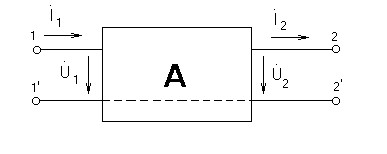
\includegraphics[width=0.8\textwidth]{./content/RIs001.jpg}
  \caption{Четырёхполюсник в системе А- параметров} \label{p:RIs001}
\end{figure}



Допустим, что два чаетырёхполюсника соединяются каскадно, тогда параметры эквивалентного четырёхполюсника определяются по формуле~(\ref{eq:2}): 

\begin{equation}
\label{eq:2}
\begin{aligned}
\begin{bmatrix} A_{11} & A_{12}\\ A_{21} & A_{22} \end{bmatrix} = \begin{bmatrix} A1_{11} & A1_{12}\\ A1_{21} & A1_{22} \end{bmatrix} \begin{bmatrix} A2_{11} & A2_{12}\\ A2_{21} & A2_{22} \end{bmatrix}
\end{aligned}
\end{equation}





Отметим, что важно соблюдать порядок расстановки матриц, который должен  соответствовать  порядку  расстановки  четырёхполюсников.  Так формула~(\ref{eq:2}) справедлива для схемы на рисунке~\ref{p:RIs002}. 

\begin{figure}[H] \centering
  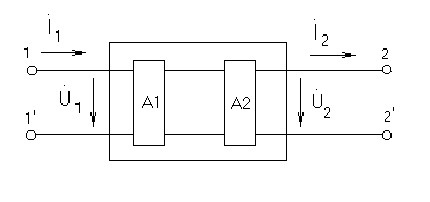
\includegraphics[width=0.8\textwidth]{./content/RIs002.jpg}
  \caption{Схема каскадного соединения четырёхполюсников} \label{p:RIs002}
\end{figure}






В  результате  таких  преобразований  получается  система  А- параметров  сложного  четырёхполюсника.  Коэффициент  передачи четырёхполюсника по напряжению рассчитывается по формуле~(\ref{eq:3}): 

\begin{equation}
\label{eq:3}
K_{U} = \frac{Z_{n}}{A_{11}Z_{n} + A_{12}}
\end{equation}

где $Z_{n}$- сопротивление на которое нагружается выход четырёхполюсника.
\\

Во  многих  случаях  (особенно  при  расчёте  фильтров  согласованной селекции)  при  расчёте  коэффициента  передачи  следует  учитывать,  что  четырёхполюсник должен быть нагружен и по входу. На рисунке~\ref{p:RIs003} показана схема, в соответствии с которой работает данная формула.  

\begin{figure}[H] \centering
  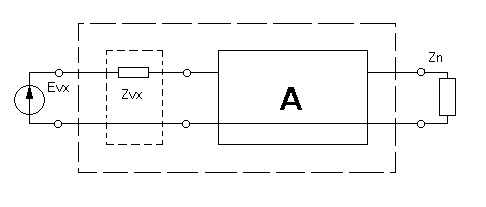
\includegraphics[width=0.8\textwidth]{./content/RIs003.jpg}
  \caption{Пояснение работы формулы~(\ref{eq:3})} \label{p:RIs003}
\end{figure}



Формула~(\ref{eq:3})  учитывает  только  идеальный источник напряжения $E_{\text{ВХ}}$  и  сопротивление  нагрузки  $Z_{n}$.  Сопротивление  $Z_{\text{VX}}$  нужно  включить  в параметры четырёхполюсника предварительно.  

Входное  и  выходное  сопротивления  рассчитываются  по  следующим формулам:  

\begin{equation}
\label{eq:4}
Z_{\text{VX}} = \frac{A_{11}Z_{n} + A_{12}}{A_{21}Z_{n} + A_{22}}
\end{equation}


\begin{equation}
\label{eq:5}
Z_{\text{ВЫХ}} = \frac{A_{22}Z_{\text{VX}} + A_{12}}{A_{21}Z_{\text{VX}}+ A_{11}}
\end{equation}

Как  было  сказано  выше,  сложный  четырёхполюсник  можно представить  в  виде  каскадного  соединения  простых  четырёхполюсников. Определим  А-параметры  некоторых  простых  четырёхполюсников.  На рисунке~\ref{p:RIs004}  приведены  схемы  простых  четырёхполюсников  и 
соответствующие им матрицы А-параметров. 


\begin{figure}[H] \centering
  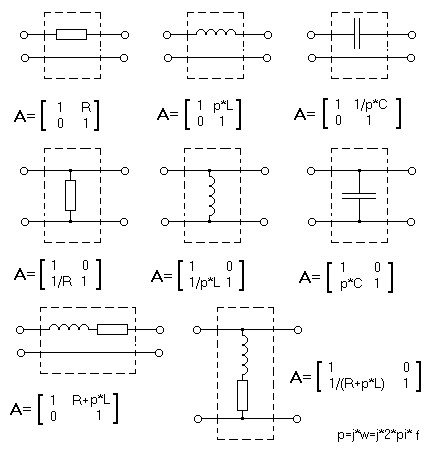
\includegraphics[width=0.8\textwidth]{./content/RIs004.jpg}
  \caption{Матрицы А- параметров четырёхполюсников} \label{p:RIs004}
\end{figure}










\section{Моделирование фильтра сосредоточенной селекции}
\sectionmark{Моделирование фильтра сосредоточенной селекции}


В  качестве  примера  применения  данного  метода  рассчитаем  АЧХ  и ФЧХ  фильтра  сосредоточенной  селекции.  Точные  формулы  для  расчёта элементов звена фильтра а также схема звена приведены в \cite{Sivers}, c. 283.  

Программа написана в среде MATLAB/OCTAVE  и оформлена в виде .m –файла.  Листинг  данной  программы  приведён  в  приложении~А,  а  алгоритм работы на рисунке~\ref{p:RIs005}. 



\begin{figure}[H] \centering
  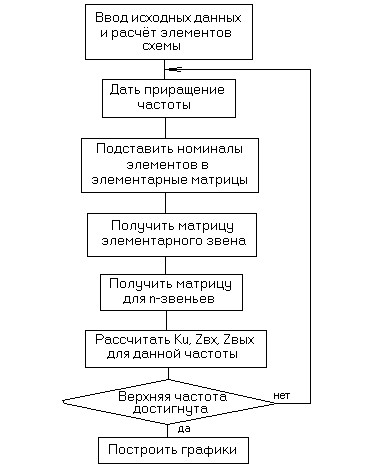
\includegraphics[width=0.8\textwidth]{./content/RIs005.jpg}
  \caption{Алгоритм работы программы расчёта ФСС} \label{p:RIs005}
\end{figure}








На  рисунках~\ref{p:RIs006}, \ref{p:RIs007}, \ref{p:RIs008}  приведены  графики,  полученные  с  помощью данного метода.


\begin{figure}[H] \centering
  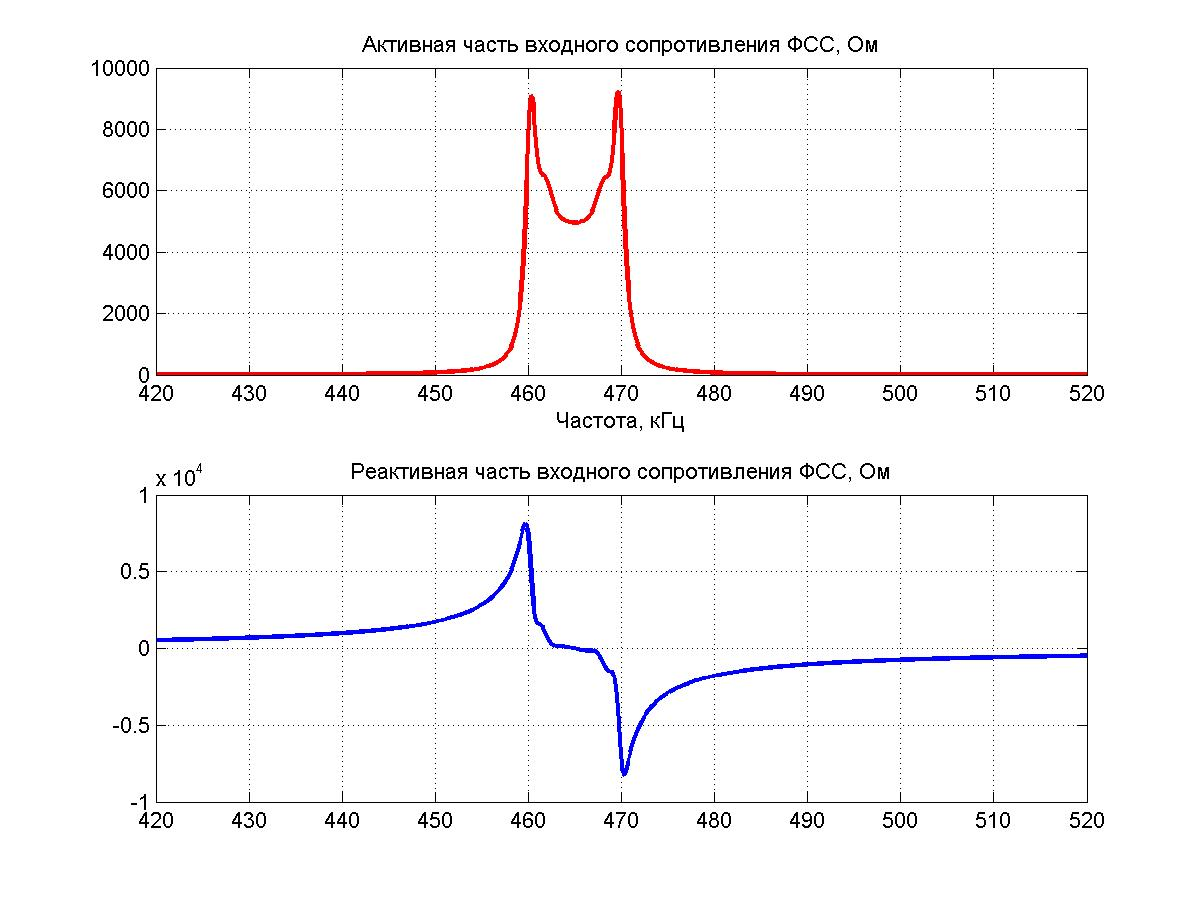
\includegraphics[width=0.8\textwidth]{./content/RIs006.jpg}
  \caption{Входное сопротивление ФСС} \label{p:RIs006}
\end{figure}


\begin{figure}[H] \centering
  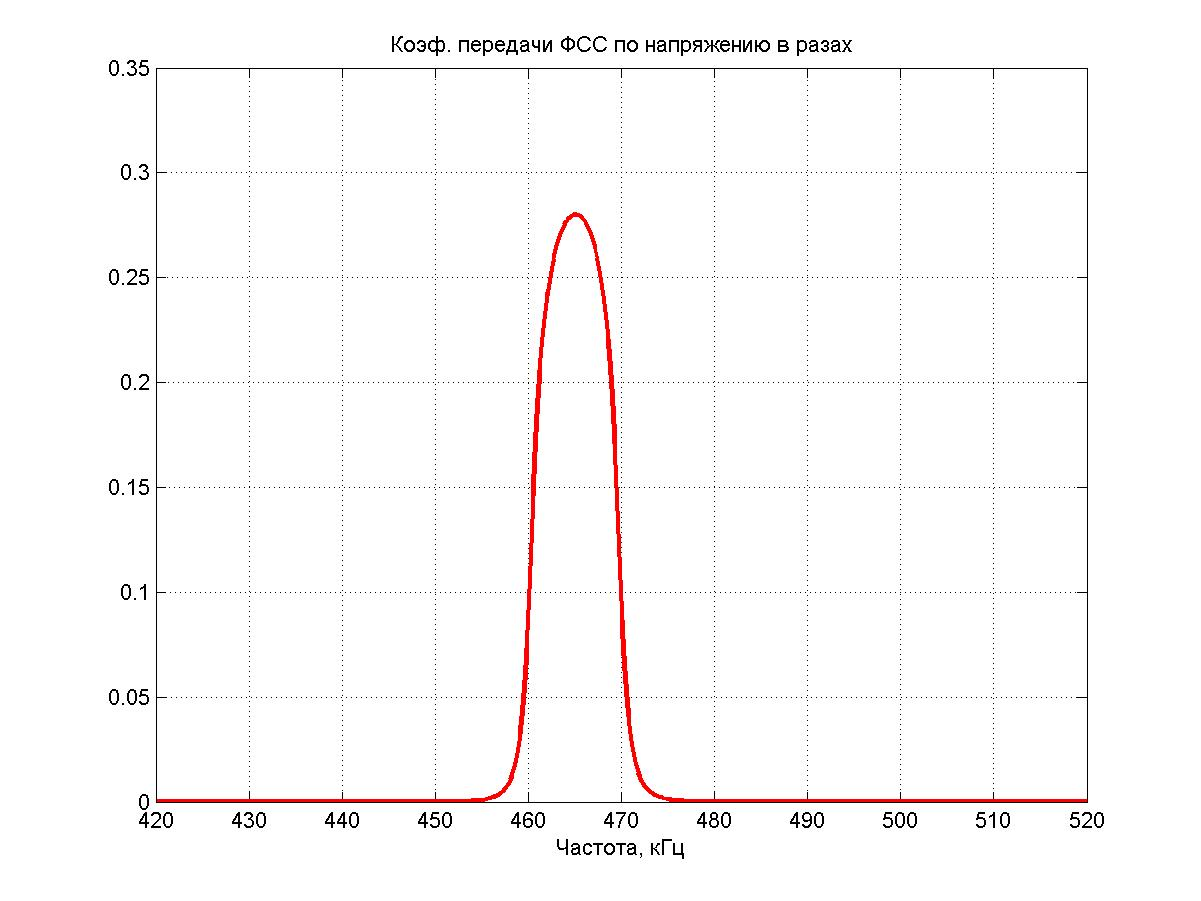
\includegraphics[width=0.8\textwidth]{./content/RIs007.jpg}
  \caption{Коэффициент передачи по напряжению ФСС} \label{p:RIs007}
\end{figure}


\begin{figure}[H] \centering
  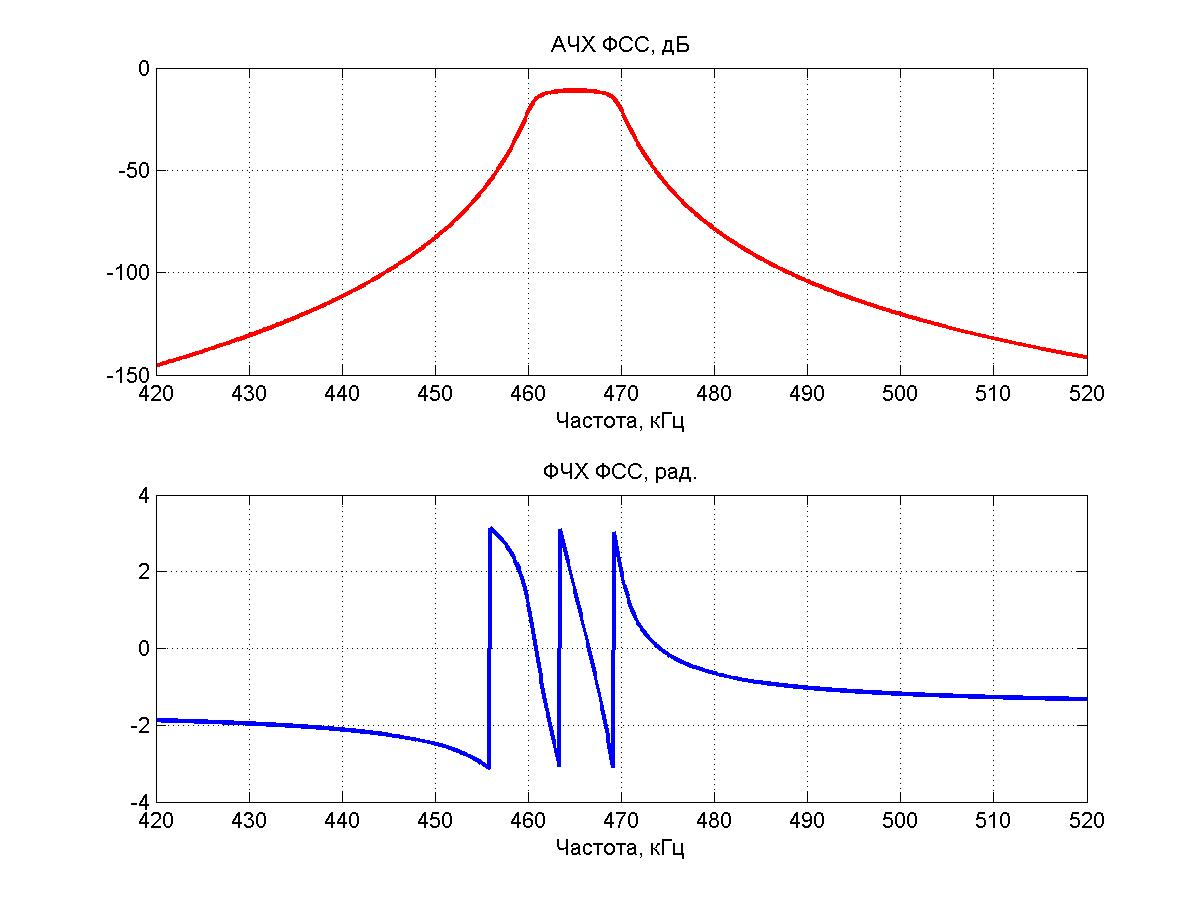
\includegraphics[width=0.8\textwidth]{./content/RIs008.jpg}
  \caption{АЧХ и ФЧХ фильтра сосредоточенной селекции} \label{p:RIs008}
\end{figure}






%%%%%%%%%%%%%%%%%%%%%%%%%%%%%%%%%%%%%%%

\section{Моделирование входной цепи}
\sectionmark{Моделирование входной цепи}

Рассмотрим  некоторые  особенности  применения  данного  метода.  В литературе обычно пользуются моделями четырёхполюсников в системе Y-параметров.  Ниже  приведены  формулы  для  пересчёта  из  одной  системы параметров в другую:  

\begin{equation}
\label{eq:6}
\begin{aligned}
 \begin{cases}
\mid Y\mid = Y_{11}Y_{22} - Y_{12}Y_{21}\\
\\
A_{11} = - \dfrac{Y_{22}}{Y_{21}}\\
\\
A_{12} = - \dfrac{1}{Y_{21}}\\
\\
A_{21} = - \dfrac{\mid Y\mid}{Y_{21}}\\
\\
A_{22} = - \dfrac{Y_{11}}{Y_{21}}\\
 \end{cases}
\end{aligned}
\end{equation}


\begin{equation}
\label{eq:7}
\begin{aligned}
 \begin{cases}
\mid A\mid = A_{11}A_{22} - A_{12}A_{21}\\
\\
Y_{11} = \dfrac{A_{22}}{A_{12}}\\
\\
Y_{12} = - \dfrac{\mid A\mid}{A_{12}}\\
\\
Y_{21} = - \dfrac{1}{A_{12}}\\
\\
Y_{22} = \dfrac{A_{11}}{A_{12}}\\
 \end{cases}
\end{aligned}
\end{equation}


Система  Y-  параметров  также  полезна  тем,  что  допускает  параллельное соединение  четырёхполюсников.  Ниже  приведены  формулы  и  схема, поясняющая их работу:


\begin{equation}
\label{eq:8}
\begin{aligned}
\begin{bmatrix} Y_{11} & Y_{12}\\ Y_{21} & Y_{22} \end{bmatrix} = \begin{bmatrix} Y1_{11} & Y1_{12}\\ Y1_{21} & Y1_{22} \end{bmatrix} +\begin{bmatrix} Y2_{11} & Y2_{12}\\ Y2_{21} & Y2_{22} \end{bmatrix}
\end{aligned}
\end{equation}


\begin{figure}[H] \centering
  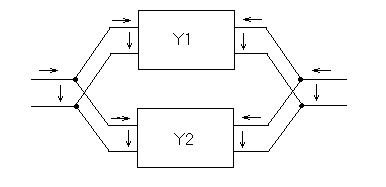
\includegraphics[width=0.8\textwidth]{./content/RIs009.jpg}
  \caption{Параллельное соединение четырёхполюсников} \label{p:RIs009}
\end{figure}


Применим  данные  формулы  для  расчёта  входной  цепи  приёмника  с индуктивно-емкостной  связью  с  антенной.  Данная  схема  представлена  на рисунке~\ref{p:RIs010}. 


\begin{figure}[H] \centering
  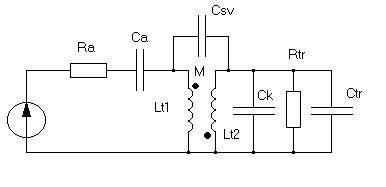
\includegraphics[width=0.8\textwidth]{./content/RIs010.jpg}
  \caption{Схема входной цепи с индуктивно-емкостной связью} \label{p:RIs010}
\end{figure}


Из рисунка~\ref{p:RIs010} видно, что в цепи присутствует трансформатор. Нужно обратить  внимание  на  включение  обмоток  трансформатора.  На  рисунке~\ref{p:RIs011} приведены  схемы  трансформаторных  элементов  с  разным  включением обмоток. 


\begin{figure}[H] \centering
  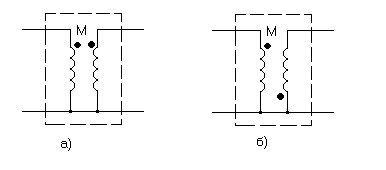
\includegraphics[width=0.8\textwidth]{./content/RIs011.jpg}
  \caption{Схемы трансформаторных элементов} \label{p:RIs011}
\end{figure}

Уравнения  схемы  на  рисунке~\ref{p:RIs011}.а  в  системе  Y-параметров приведены ниже: 



\begin{equation}
\label{eq:9}
\begin{aligned}
\begin{bmatrix} I_{1}\\ \\ I_{2} \end{bmatrix} = 
\begin{bmatrix} \dfrac{L_{2} p}{L_{1} L_{2} p^{2} - (p M)^{2}} &
                           \dfrac{-M p}{L_{1} L_{2} p^{2} - (p M)^{2}}\\ 
						      \dfrac{-M p}{L_{1} L_{2} p^{2} - (p M)^{2}} &
							  \dfrac{L_{1} p}{L_{1} L_{2} p^{2} - (p M)^{2}}
\end{bmatrix}
\begin{bmatrix} U_{1}\\ \\  U_{2} \end{bmatrix}
\end{aligned}
\end{equation}




Уравнения  для  схемы  на  рисунке~\ref{p:RIs011}.б  легко  получить,  произведя подстановку: 

\begin{equation}
\label{eq:10}
\begin{aligned}
 \begin{cases}
I_{2} \to (- I_{2})\\
U_{2} \to (- U_{2})
 \end{cases}
\end{aligned}
\end{equation}

Таким образом, уравнения для случая~\ref{p:RIs011}.б примут вид: 


\begin{equation}
\label{eq:11}
\begin{aligned}
\begin{bmatrix} I_{1}\\ \\ I_{2} \end{bmatrix} = 
\begin{bmatrix} \dfrac{L_{2} p}{L_{1} L_{2} p^{2} - (p M)^{2}} &
                           \dfrac{M p}{L_{1} L_{2} p^{2} - (p M)^{2}}\\ 
						      \dfrac{M p}{L_{1} L_{2} p^{2} - (p M)^{2}} &
							  \dfrac{L_{1} p}{L_{1} L_{2} p^{2} - (p M)^{2}}
\end{bmatrix}
 \begin{bmatrix} U_{1}\\ \\  U_{2} \end{bmatrix}
\end{aligned}
\end{equation}


Для получения Y- параметров конденсатора $C_{SV}$ на рисунке~\ref{p:RIs010} нужно воспользоваться  матрицей  А-  параметров  с  рисунка~\ref{p:RIs004}  и  формулами~(\ref{eq:7}). Воспользовавшись~(\ref{eq:8})  получим  матрицу  Y-  параметров  параллельного соединения трансформатора и конденсатора $C_{SV}$. Далее  перейдя с помощью~(\ref{eq:6}) в систему А- параметров, достроим эквивалентный четырёхполюсник для всей цепи.  


В  приложении~\ref{app:matlab_vplc}  приведён  листинг  программы,  вычисляющей параметры  цепи  на  рисунке~\ref{p:RIs010}  при  известных  номиналах  элементов.  К особенности данной программы относится то, что она вычисляет семейство коэффициентов  передачи  по  напряжению, что достигнуто с помощью двух циклов,  один  из  которых  вложен  в  другой.  Один  отвечает  за  изменение частоты, а другой за изменение номинала конденсатора переменной ёмкости. Ниже на рисунке~\ref{p:RIs012} приведено семейство АЧХ в рабочем диапазоне частот. 


\begin{figure}[H] \centering
  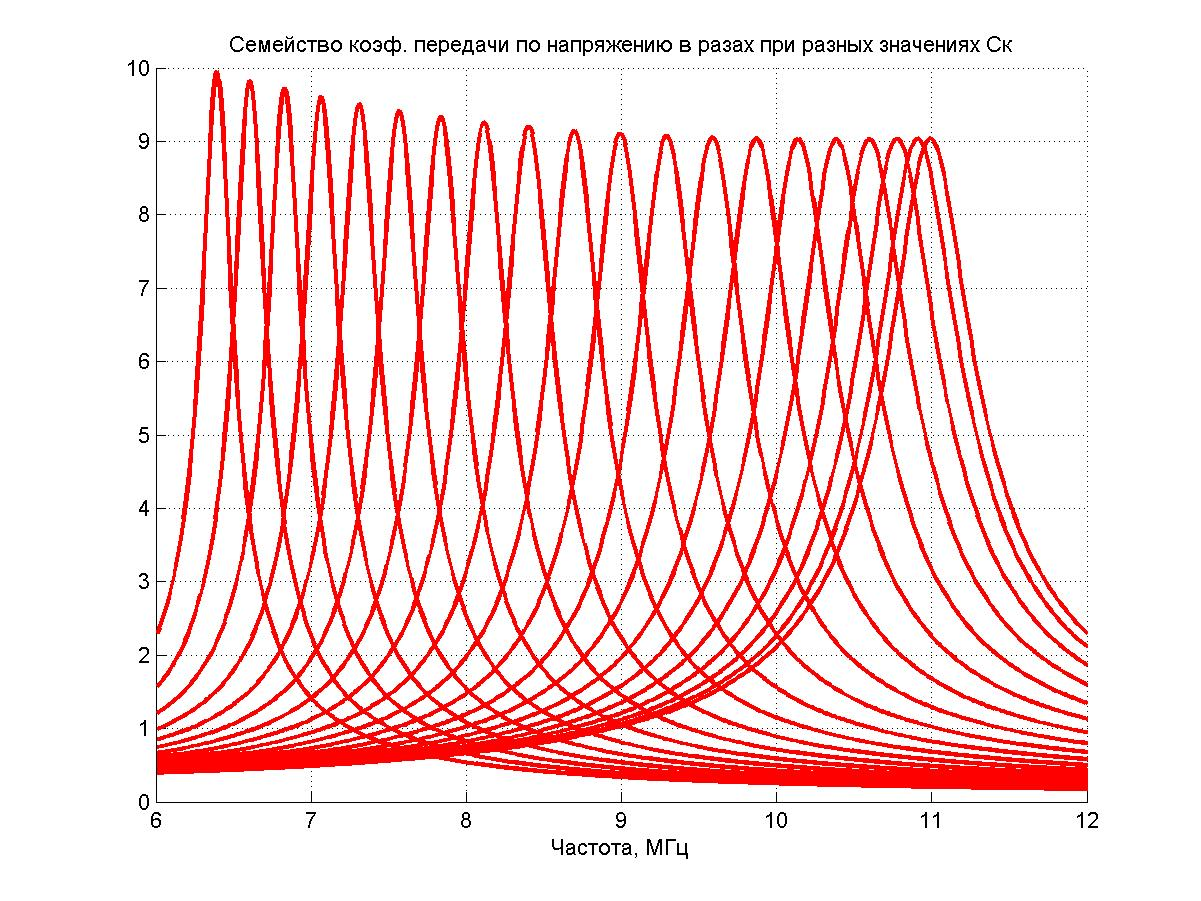
\includegraphics[width=0.8\textwidth]{./content/RIs012.jpg}
  \caption{АЧХ для схемы с рисунка~\ref{p:RIs010}} \label{p:RIs012}
\end{figure}


Отметим, что при расчёте АЧХ было использовано  завышенное активное входное сопротивление транзистора (порядка 10~кОм), что и послужило причиной высокого коэффициента передачи. Нужно сказать, что данная схема предназначена для применения совместно с лампами а не с транзисторами, что легко проиллюстрировать, построив график изменения выходного сопротивления от частоты при фиксированном значении КПЕ (рисунок~\ref{p:RIs013}). 


\begin{figure}[H] \centering
  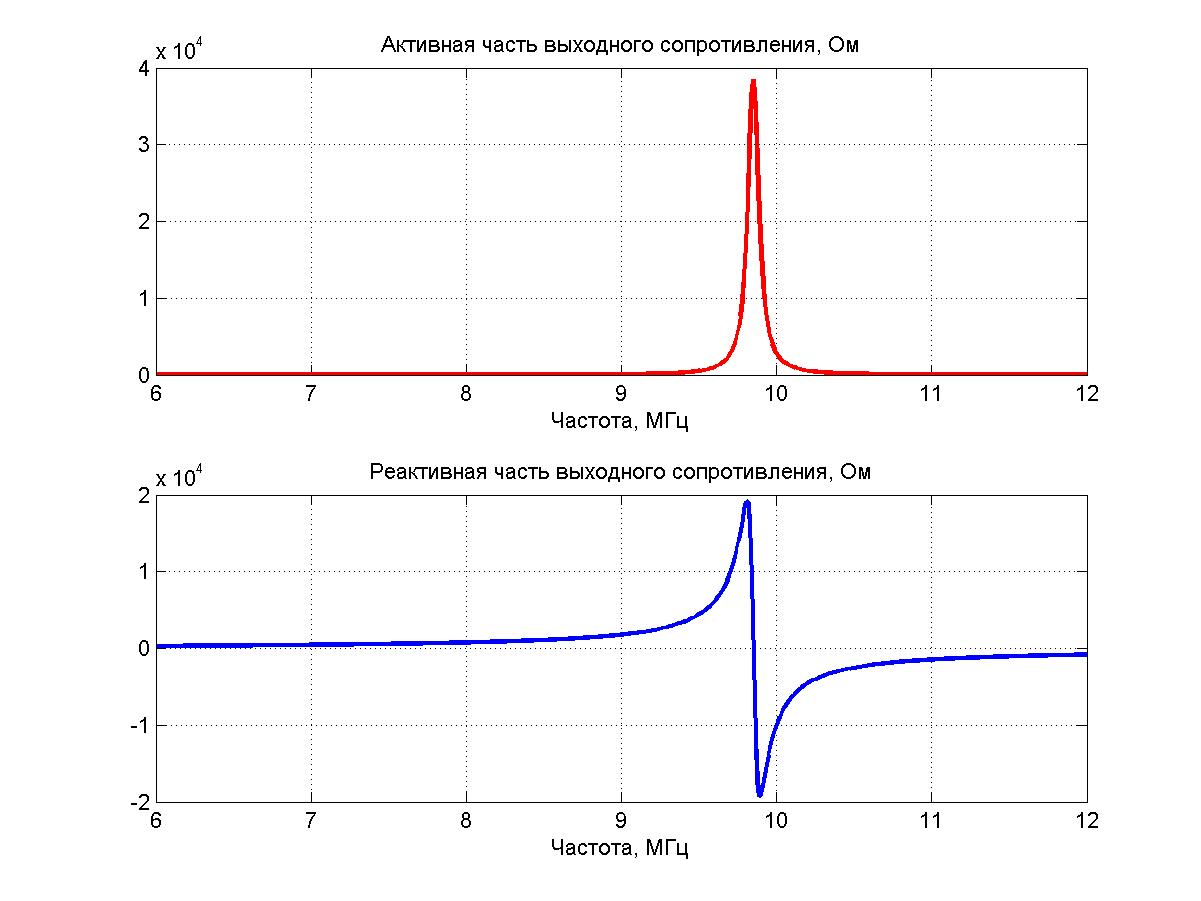
\includegraphics[width=0.8\textwidth]{./content/RIs013.jpg}
  \caption{Выходное сопротивление схемы с рисунка~\ref{p:RIs010}} \label{p:RIs013}
\end{figure}



Нужно  сказать,  что  в  рассмотренном  примере  использовалась идеализированная  модель  трансформатора  так  как  в  ней  не  учитывались потери в обмотках. В ниже приведённых формулах для схемы на рисунке~\ref{p:RIs011}.а учтены потери в обмотках:  


\begin{equation}
\label{eq:12}
\small
\begin{aligned}
\begin{bmatrix} I_{1}\\ \\ I_{2} \end{bmatrix}= 
\begin{bmatrix} \dfrac{r_{2} + L_{2} p}{(r_{1} + L_{1} p) (r_{2} + L_{2} p) - (p M)^{2}} &
                           \dfrac{-M p}{(r_{1} + L_{1} p) (r_{2} + L_{2} p) - (p M)^{2}}\\ 
						      \dfrac{-M p}{(r_{1} + L_{1} p) (r_{2} + L_{2} p) - (p M)^{2}} &
							  \dfrac{r_{1} + L_{1} p}{(r_{1} + L_{1} p) (r_{2} + L_{2} p) - (p M)^{2}}
\end{bmatrix}
 \begin{bmatrix} U_{1}\\ \\  U_{2} \end{bmatrix}
\end{aligned}
\normalsize
\end{equation}



%%%%%%%%%%%%%%%%%%%%%%%%%%%%%%%%%%%%%%

\section{Вопросы  моделирования сложных цепей}
\sectionmark{Вопросы  моделирования сложных цепей}
 
  
Как  известно,  активный  элемент  можно  рассматривать  как невзаимный  четырёхполюсник, то есть  в  случае  $Y_{12}\ne Y_{21}$  Y-  параметров. 
Данная  модель  рассмотрена  во  многих  книгах  и  может  применяться  при компьютерном  расчёте без внесения в нё каких-либо изменений.
 
 
 Рассмотрим  случай  индуктивности  с  отводом.  Схема  приведена  на 
рисунке~\ref{p:RIs014}. 
 
 
 \begin{figure}[H] \centering
  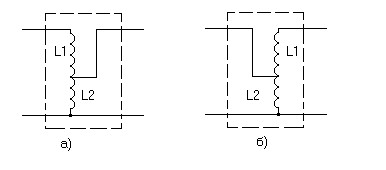
\includegraphics[width=0.8\textwidth]{./content/RIs014.jpg}
  \caption{Индуктивность с отводом} \label{p:RIs014}
\end{figure}
 
Для случая на рисунке~\ref{p:RIs014}.а получаем: 

\begin{equation}
\label{eq:13}
\footnotesize
\begin{aligned}
\begin{bmatrix} I_{1}\\ \\ I_{2} \end{bmatrix} = 
\begin{bmatrix} \dfrac{L_{2} p}{L_{2}(L_{1} + L_{2} + 2M)p^{2} - \bigl((L_{2} + M)p\bigr)^{2}} &
                           \dfrac{-(L_{2}+M)p}{L_{2}(L_{1} + L_{2} + 2M)p^{2} - \bigl((L_{2} + M)p\bigr)^{2}}\\ 
						      \dfrac{-(L_{2}+M)p}{L_{2}(L_{1} + L_{2} + 2M)p^{2} - \bigl((L_{2} + M)p\bigr)^{2}} &
							  \dfrac{(L_{1}+ L_{2} + 2M)p}{L_{2}(L_{1} + L_{2} + 2M)p^{2} - \bigl((L_{2} + M)p\bigr)^{2}}
\end{bmatrix}
\begin{bmatrix} U_{1}\\ \\  U_{2} \end{bmatrix}
\end{aligned}
\normalsize
\end{equation}


Для случая на рисунке~\ref{p:RIs014}.б формулы получаются при подстановке в (\ref{eq:13}) следующих соотношений: 

\begin{equation}
\label{eq:14}
\begin{aligned}
 \begin{cases}
I_{1} \to I_{2}\\
I_{2} \to I_{1}\\
U_{1} \to U_{2}\\
U_{2} \to U_{1}\\
 \end{cases}
\end{aligned}
\end{equation}



В результате :


\begin{equation}
\label{eq:15}
\footnotesize
\begin{aligned}
\begin{bmatrix} I_{1}\\ \\ I_{2} \end{bmatrix} = 
\begin{bmatrix} \dfrac{(L_{1} + L_{2} + 2M)p}{L_{2}(L_{1} + L_{2} + 2M)p^{2} - \bigl((L_{2} + M)p\bigr)^{2}} &
                           \dfrac{-(L_{2}+M)p}{L_{2}(L_{1} + L_{2} + 2M)p^{2} - \bigl((L_{2} + M)p\bigr)^{2}}\\ 
						      \dfrac{-(L_{2}+M)p}{L_{2}(L_{1} + L_{2} + 2M)p^{2} - \bigl((L_{2} + M)p\bigr)^{2}} &
							  \dfrac{L_{2}p}{L_{2}(L_{1} + L_{2} + 2M)p^{2} - \bigl((L_{2} + M)p\bigr)^{2}}
\end{bmatrix}
\begin{bmatrix} U_{1}\\ \\  U_{2} \end{bmatrix}
\end{aligned}
\normalsize
\end{equation}



При  анализе  большинства  схем  резонансных  усилителей  требуется модель колебательного контура с двумя отводами от индуктивности. Схема такого контура приведена на рисунке~\ref{p:RIs015}. 

 \begin{figure}[H] \centering
  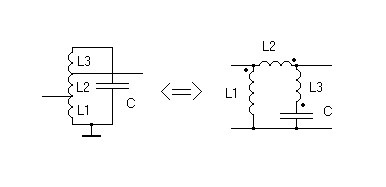
\includegraphics[width=0.8\textwidth]{./content/RIs015.jpg}
  \caption{Колебательный контур с отводами от индуктивности } \label{p:RIs015}
\end{figure}

К  сожалению,  из-за  сложности  формул  (необходимости  учёта  не только  индуктивностей  L1, L2, L3  но  и  взаимоиндуктивностей  M12,  M13, M23)  в  данной  работе  не  были  получены  Y-  параметры  данного четырёхполюсника. 



%%%%%%%%%%%%%%%%%%%%%%%%%%%%%%%%%%%%%%%
 
\section*{Заключение}
\sectionmark{Заключение}

Как  видно,  данный  метод  анализа  имеет  как  сильные  так  и  слабые стороны. К последним относятся трудность получения параметров сложных четырёхполюсников,  внимательность  и  приблизительное  предвидение результата  моделирования  при  составлении  моделей.  Нужно  сказать,  что современныё  пакеты  моделирования  электронных  схем  обладают  гораздо 
большими возможностями анализа.  

К  сильным  сторонам  относится  открытость  алгоритма  анализа, возможности  задания  сложных  зависимостей  номиналов  элементов  от частоты,  возможность  проведения  оптимизации  сразу  по  нескольким параметрам. 











